%%%%%%%%%%%%%%%%%%%%%%%%%%%%%%%%%%%%%%%%%
% Article EcoFoG
% Version 2.1 (23/10/2017)
%
% adapté de :
% Stylish Article
% LaTeX Template
% Version 1.0 (31/1/13)
%
% This template has been downloaded from:
% http://www.LaTeXTemplates.com
%
% Original author:
% Mathias Legrand (legrand.mathias@gmail.com)
%
% License:
% CC BY-NC-SA 3.0 (http://creativecommons.org/licenses/by-nc-sa/3.0/)
%
%%%%%%%%%%%%%%%%%%%%%%%%%%%%%%%%%%%%%%%%%


%----------------------------------------------------------------------------------------
%	PACKAGES AND OTHER DOCUMENT CONFIGURATIONS
%----------------------------------------------------------------------------------------

\documentclass[fleqn,10pt]{ArtEcoFoG} % Document font size and equations flushed left

\setcounter{tocdepth}{3} % Show only three levels in the table of contents section: sections, subsections and subsubsections


% Pandoc environments
\usepackage{framed}
\usepackage{fancyvrb}
\providecommand{\tightlist}{%
  \setlength{\itemsep}{0pt}\setlength{\parskip}{0pt}}
\newcommand{\VerbBar}{|}
\newcommand{\VERB}{\Verb[commandchars=\\\{\}]}
\DefineVerbatimEnvironment{Highlighting}{Verbatim}{commandchars=\\\{\}, fontsize=\scriptsize} % Code R
\definecolor{shadecolor}{RGB}{248,248,248}
\newenvironment{Shaded}{\begin{snugshade}}{\end{snugshade}}
\newcommand{\KeywordTok}[1]{\textcolor[rgb]{0.13,0.29,0.53}{\textbf{{#1}}}}
\newcommand{\DataTypeTok}[1]{\textcolor[rgb]{0.13,0.29,0.53}{{#1}}}
\newcommand{\DecValTok}[1]{\textcolor[rgb]{0.00,0.00,0.81}{{#1}}}
\newcommand{\BaseNTok}[1]{\textcolor[rgb]{0.00,0.00,0.81}{{#1}}}
\newcommand{\FloatTok}[1]{\textcolor[rgb]{0.00,0.00,0.81}{{#1}}}
\newcommand{\ConstantTok}[1]{\textcolor[rgb]{0.00,0.00,0.00}{{#1}}}
\newcommand{\CharTok}[1]{\textcolor[rgb]{0.31,0.60,0.02}{{#1}}}
\newcommand{\SpecialCharTok}[1]{\textcolor[rgb]{0.00,0.00,0.00}{{#1}}}
\newcommand{\StringTok}[1]{\textcolor[rgb]{0.31,0.60,0.02}{{#1}}}
\newcommand{\VerbatimStringTok}[1]{\textcolor[rgb]{0.31,0.60,0.02}{{#1}}}
\newcommand{\SpecialStringTok}[1]{\textcolor[rgb]{0.31,0.60,0.02}{{#1}}}
\newcommand{\ImportTok}[1]{{#1}}
\newcommand{\CommentTok}[1]{\textcolor[rgb]{0.56,0.35,0.01}{\textit{{#1}}}}
\newcommand{\DocumentationTok}[1]{\textcolor[rgb]{0.56,0.35,0.01}{\textbf{\textit{{#1}}}}}
\newcommand{\AnnotationTok}[1]{\textcolor[rgb]{0.56,0.35,0.01}{\textbf{\textit{{#1}}}}}
\newcommand{\CommentVarTok}[1]{\textcolor[rgb]{0.56,0.35,0.01}{\textbf{\textit{{#1}}}}}
\newcommand{\OtherTok}[1]{\textcolor[rgb]{0.56,0.35,0.01}{{#1}}}
\newcommand{\FunctionTok}[1]{\textcolor[rgb]{0.00,0.00,0.00}{{#1}}}
\newcommand{\VariableTok}[1]{\textcolor[rgb]{0.00,0.00,0.00}{{#1}}}
\newcommand{\ControlFlowTok}[1]{\textcolor[rgb]{0.13,0.29,0.53}{\textbf{{#1}}}}
\newcommand{\OperatorTok}[1]{\textcolor[rgb]{0.81,0.36,0.00}{\textbf{{#1}}}}
\newcommand{\BuiltInTok}[1]{{#1}}
\newcommand{\ExtensionTok}[1]{{#1}}
\newcommand{\PreprocessorTok}[1]{\textcolor[rgb]{0.56,0.35,0.01}{\textit{{#1}}}}
\newcommand{\AttributeTok}[1]{\textcolor[rgb]{0.77,0.63,0.00}{{#1}}}
\newcommand{\RegionMarkerTok}[1]{{#1}}
\newcommand{\InformationTok}[1]{\textcolor[rgb]{0.56,0.35,0.01}{\textbf{\textit{{#1}}}}}
\newcommand{\WarningTok}[1]{\textcolor[rgb]{0.56,0.35,0.01}{\textbf{\textit{{#1}}}}}
\newcommand{\AlertTok}[1]{\textcolor[rgb]{0.94,0.16,0.16}{{#1}}}
\newcommand{\ErrorTok}[1]{\textcolor[rgb]{0.64,0.00,0.00}{\textbf{{#1}}}}
\newcommand{\NormalTok}[1]{{#1}}
\usepackage{longtable,booktabs}
\usepackage{caption}
% These lines are needed to make table captions work with longtable:
\makeatletter
\def\fnum@table{\tablename~\thetable}
\makeatother
% longtable 2 columns
% https://tex.stackexchange.com/questions/161431/how-to-solve-longtable-is-not-in-1-column-mode-error
\makeatletter
\let\oldlt\longtable
\let\endoldlt\endlongtable
\def\longtable{\@ifnextchar[\longtable@i \longtable@ii}
\def\longtable@i[#1]{\begin{figure}[t]
\onecolumn
\begin{minipage}{0.5\textwidth}\scriptsize
\oldlt[#1]
}
\def\longtable@ii{\begin{figure}[t]
\onecolumn
\begin{minipage}{0.5\textwidth}\scriptsize
\oldlt
}
\def\endlongtable{\endoldlt
\end{minipage}
\twocolumn
\end{figure}}
\makeatother

\usepackage{graphicx,grffile}
\makeatletter
\def\maxwidth{\ifdim\Gin@nat@width>\linewidth\linewidth\else\Gin@nat@width\fi}
\def\maxheight{\ifdim\Gin@nat@height>\textheight0.8\textheight\else\Gin@nat@height\fi}
\makeatother
% Scale images if necessary, so that they will not overflow the page
% margins by default, and it is still possible to overwrite the defaults
% using explicit options in \includegraphics[width, height, ...]{}
\setkeys{Gin}{width=\maxwidth,height=\maxheight,keepaspectratio}

% User-adder preamble
\usepackage{textcomp} \DeclareUnicodeCharacter{B0}{\textdegree}
\usepackage{tabu} \usepackage{caption}
\captionsetup{justification = justified}
\renewenvironment{table}{\begin{table*}}{\end{table*}\ignorespacesafterend}
\hyphenation{bio-di-ver-si-ty sap-lings re-or-gan-i-za-tion post-dis-tur-bance dis-tur-bance}

%----------------------------------------------------------------------------------------
%	ARTICLE INFORMATION
%----------------------------------------------------------------------------------------

\JournalInfo{\ }
\Archive{\ }

\PaperTitle{Post-Disturbance Tree Community Trajectories in a Neotropical Forest} % Article title

\Authors{
Ariane MIRABEL\textsuperscript{1*}\\ Bruno Herault\textsuperscript{2}\\ Eric Marcon\textsuperscript{1}
} % Authors
\affiliation{
\textsuperscript{1}UMR EcoFoG, AgroParistech, CNRS, Cirad, INRA, Université des Antilles,
Université de Guyane.\\ \hspace{1em} Campus Agronomique, 97310 Kourou, France.\\\textsuperscript{2}INPHB, Institut National Polytechnique Félix Houphoüet-Boigny\\ \hspace{1em} Yamoussoukro, Ivory Coast.
}
\affiliation{*\textbf{Corresponding author}: ariane.mirabel@ecofog.gf, https://github.com/ArianeMirabel} % Corresponding author

\Keywords{Community Ecology, Community Diversity Determinants, Disturbance Trajectories, Intermediate Disturbance Hypothesis, Mid-term Resilience, Neotropical Forests, Taxonomic and Functional Biodiversity} % Keywords - if you don't want any simply remove all the text between the curly brackets
\newcommand{\keywordname}{Keywords} % Defines the keywords heading name

%----------------------------------------------------------------------------------------
%	ABSTRACT
%----------------------------------------------------------------------------------------

\Abstract{
Understanding the ecological rules underlying the maintenance of
tropical forests biodiversity, structure, functioning and dynamics is
urgent to anticipate their fate in the global change context. The huge
diversity of tropical forests is often assumed to be regularly reshaped
by natural disturbance yielding a diversity peak at intermediate
intensity. This intermediate disturbance hypothesis (IDH), though,
remains debated and the controversy questions the extent of community
resilience regarding their taxonomic and functional facets. To
disentangle the ecological processes driving community response to
disturbance, we analyzed the tree community trajectories over 30 years
following a disturbance gradient in a Neotropical forest. Specifically,
we examined community functional and taxonomic trajectories with regards
to diversity, composition and redundancy. Functional trajectories were
drawn based on 7 leaf, stem and life-history traits. We highlighted the
cyclic recovery of community taxonomic and functional composition. While
pre-disturbance taxonomic differences were maintained over time,
functional composition trajectories were quite similar among
communities. The IDH did predict community taxonomic diversity response
while functional diversity was enhanced whatever the disturbance
intensity. Although consistent, the recovery of community composition,
diversity and redundancy remained unachieved after 30 years. This
acknowledged the need of decades-long cycles with no disturbance to
ensure a complete recovery, and questioned tropical forest community
resilience after repeated disturbances.
}

%----------------------------------------------------------------------------------------

\begin{document}

\selectlanguage{english}

\flushbottom % Makes all text pages the same height

\maketitle % Print the title and abstract box

\tableofcontents % Print the contents section

\thispagestyle{empty} % Removes page numbering from the first page

%----------------------------------------------------------------------------------------
%	ARTICLE CONTENTS
%----------------------------------------------------------------------------------------
























\section{Introduction}\label{introduction}

Tropical forests cover large areas worldwide and represent crucial
environmental, economic and social values. They provide wood and
multiple non-timber forest products, shelter a diversified fauna,
regulate the local and regional climates, determine the cycles of
carbon, water and nutrient, and ensure cultural and human well-being.
However, the growing demand in forests products together with current
global changes increases the pressure on remaining natural forests
\citep{Morales-Hidalgo2015}. This context specifically threatens the
maintenance of community structure, composition and functioning
\citep{Anderson-Teixeira2013}. In tropical forests indeed, tree
communities are shaped and maintained by a natural disturbance regime,
specifically tree fall gaps\citep{Schnitzer2001}. This disturbance
regime is affected by the current changing context and anthropic
activities \citep{Sist2015}, so clarify community responses to
disturbance and the underlying ecological processes is crucial to
anticipate the fate of tropical forests \citep{Chazdon2003a}.

Disturbances change both biotic and abiotic environment, through
modifications in the fluxes of light, heat and water
\citep{Goulamoussene2017}, and of the interactions among species such as
competition \citep{Chesson2000}. Community response has been largely
studied through forest structural parameters such as aboveground
biomass, tree height or stem density
\citep{Piponiot2016, Rutishauser2016}. Thereafter, models based on the
observed trajectories after disturbance gave important insights into the
recovery of ecosystem processes and services \citep{Herault2018}.
Regarding community diversity and composition, however, post-disturbance
trajectories are not as thoroughly understood. It is recognized that
determined succession, mainly driven by the recruitment of pioneer and
heliophilous species, shape post-disturbance trajectories
\citep{Carreno-Rocabado2012, Poorter2016}. Community trajectories would
then rely on deterministic processes and would be predictable according
to the disturbance intensity and to the characteristics of the
pre-disturbance community. Yet, observed trajectories in diversity and
composition often deviate from predictions. Besides, although the
deterministic ecological processes at stake are identified, their
relative importance compared to stochasticity remains debated
\citep{Norden2015}. This debate translates into the validation and the
extent of the intermediate disturbance hypothesis (IDH). The IDH assumes
the predominance of deterministic processes, and predicts a maximum
species diversity after moderate disturbance intensity
\citep{Molino2001, Kariuki2006a}. Validations of the IDH remain scarce
in the long-term and often rely on the analysis of taxonomic richness
\citep{Molino2001}. Taxonomic richness alone, however, gives limited or
misleading information on forests recovery and functioning
\citep{Chaudhary2016}. More ecological-meaningful analysis would couple
richness with species evenness, which reveals the changes in the species
abundance distribution, and (ii)species composition, which is crucial
for conservation issues \citep{Lavorel2002, Bellwood2006}. Furthermore,
a functional approach accounting for species biological attributes would
directly link community diversity, composition and redundancy to
ecosystem functioning and to its environmental constraints
\citep{Violle2007b, Baraloto2012a}. In that respect, the functional
trait-based approach that focus on major traits related to species
ecology and mediate species performance in a given environment was
successfully adopted \citep{Diaz2005}. For instance, the functional
approach revealed in tropical rainforests the deterministic processes
entailing, after disturbance, a functional shift from a dominance of
``conservative'' slow-growing species dealing with scarce resources to
``acquisitive'' fast-growing species with rapid and efficient use of
abundant resources \citep{Reich2014, Herault2011}. This shift is
translated into the trajectories of key functional traits related to
resource acquisition (leaf and stem traits) and life-history traits
(seed mass, maximum size)
\citep{Wright2004, TerSteege2006, Westoby2006a, Chave2009b}. Eventually,
a complete overview of community response to disturbance would encompass
the changes in functional redundancy, that quantifies the amount of
shared trait values among species \citep{Carmona2016}. The high
functional redundancy of hyper-diverse tropical forests
\citep{Bellwood2006} mitigates the impacts of species removal on
ecosystem functioning and determines community resilience after
disturbance \citep{Elmqvist2003, Diaz2005}.

Improve the understanding of diversity and composition response to
disturbance would then require to combine taxonomic and functional
diversity and composition metrics that is not often provided
\citep[\citet{Mouillot2013}]{Carreno-Rocabado2012}. Long term monitoring
provided trajectories over several decades would allow to put in
perspectives the existing studies that often correspond to
chronosequence studies \citep{Chazdon2007} or cover 10 or 15 years after
disturbance \citep{Carreno-Rocabado2012}.

In this study, we monitored over 30 years the response of 75 ha of
Neotropical forest plots set up on a gradient of disturbance intensity,
from 10 to 60\% of ecosystem above-ground biomass (AGB) loss. We made
use of a large functional traits database encompassing major leaf, stem
and life-history traits in order to draw the taxonomic and functional
trajectories in terms of richness, evenness, composition and redundancy.
From post-disturbance trajectories (i) we determined the taxonomic and
functional translation post-disturbance succession at community scale.
(ii) we validated the importance of deterministic processes in community
response to disturbance. We defined th interplay of deterministic and
stochastic processes along time, which allowed discussing the IDH. (iii)
examined community recovery time.

\section{Material and Methods}\label{material-and-methods}

\subsection{Study site}\label{study-site}

Paracou station in French Guiana (5\textdegree 18'N and
52\textdegree 53'W) is located in a lowland tropical rain forest in a
tropical wet climate with mean annual temperature of 26\textdegree C,
mean annual precipitation averaging 2980 mm.y\textsuperscript{-1} (30-y
period) and a 3-month dry season (\textless{} 100
mm.month\textsuperscript{-1}) from mid-August to mid-November, and a
one-month dry season in March \citep{Wagner2011}. Elevation ranges
between 5 and 50 m and soils correspond to thin acrisols over a layer of
transformed saprolite with low permeability which produces lateral
drainage during heavy rains.

The experiment is a network of 12 6.25 ha plots that underwent a
disturbance gradient of three logging, thinning and fuelwood cutting
treatments (Table \ref{tab:Tab1}) according to a randomized plot design
with three replicate blocks of four plots. The disturbance corresponds
to an intensity gradient. For treatment 1 (T1) 10 trees of commercial
species (of a diameter at 1.3 m height (DBH) equal or above 50 cm) were
felled per hectare. For treatment 2 (T2) 10 trees/ha of commercial
species (DBH \(\geq\) 50 cm) were felled and 30 trees/ha of non-valuable
species (DBH \(\geq\) 40 cm) were removed by poison girdling. For
treatment 3 (T3) 10 trees/ha of commercial species (DBH \(\geq\) 50 cm)
were felled and 30 trees/ha of non-valuable species (15 with DBH
\(\geq\) 50 cm and 15 with DBH \(\geq\) 40 cm) were removed by poison
girdling \citep{Schmitt1990}. Disturbance intensity was measured as the
percentage of aboveground biomass (\%AGB) lost between the first
inventory in 1984 and five years after disturbance \citep{Piponiot2016}
estimated with the BIOMASS R package \citep{Biomass2018}.

\begin{table}

\caption{\label{tab:Tab1}Intervention table, summary of the disturbance intensity for the 4 plot treatments in Paracou.}
\centering
\begin{tabu} to \linewidth {>{\raggedright}X>{\raggedright}X>{\raggedright}X>{\raggedright}X>{\raggedright}X}
\toprule
Treatment & Timber & Thinning & Fuelwood & \%AGB lost\\
\midrule
Control & - & - & - & 0\\
T1 & DBH $\geq$ 50 cm, commercial species, $\approx$ 10   $trees.ha^{-1}$ & - & - & $[12-33]$\\
T2 & DBH $\geq$ 50 cm, commercial species, $\approx$ 10  $trees.ha^{-1}$ & DBH $\geq$ 40 cm, non-valuable species, $\approx$ 30   $trees.ha^{-1}$ & - & $[33-56]$\\
T3 & DBH $\geq$ 50 cm, commercial species, $\approx$ 10  $trees.ha^{-1}$ & DBH $\geq$ 50 cm, non-valuable species, $\approx$ 15  $trees.ha^{-1}$ & 40 cm $\leq$ DBH $\leq$ 50 cm, non-valuable species,\ $\approx$ 15 $trees.ha^{-1}$ & $[35-56]$\\
\bottomrule
\end{tabu}
\end{table}

\subsection{Inventories protocol and dataset
collection}\label{inventories-protocol-and-dataset-collection}

The study site corresponds to a tropical rainforest typical of the
Guiana Shield with a dominance of \emph{Fabaceae},
\emph{Chrysobalanaceae}, \emph{Lecythidaceae} and \emph{Sapotaceae}. In
the 12 experimental plots, all trees above 10 cm DBH have been mapped
and measured annually since 1984. Trees are first identified with a
vernacular name assigned by the forest worker team, and afterward with a
scientific name assigned by botanists during regular botanical
campaigns. In 1984, specific vernacular names were given to 62
commercial or common species whereas more infrequent ones were
identified under general identifiers only distinguishing trees and
palms. From 2003, botanical campaigns have been conducted every 5 to 6
years to identify all trees at the species level but identification
levels still varied among plots and campaigns.

This variability of protocols in time raised methodological issues as
vernacular names usually correspond to different botanical species. This
resulted in significant taxonomic uncertainty that had to be propagated
to composition and diversity metrics. The uncertainty propagation was
done through a Bayesian framework reconstituting complete inventories at
genus level from real incomplete ones on the basis of
vernacular/botanical names association. Vernacular names were replaced
through multinomial trials based on the association probability
\(\big[\alpha_1, \alpha_2,..., \alpha_V\big]\) observed across all
inventories between each vernacular name \emph{v} and all species
\(\big[s_1, s_2,..., s_N\big]\):

\begin{align}
M_v\Big(\big[s_1, s_2,..., s_N\big],\big[\alpha_1, \alpha_2,..., \alpha_V\big]\Big) \nonumber
\end{align}

See Supplementary Materials -Fig. S1 and \citet{Aubry-Kientz2013} for
the detailed methodology.

Six functional traits representing leaf economics (leaf thickness,
toughness, total chlorophyll content and specific leaf area) and stem
economics (wood specific gravity and bark thickness), and life-history
traits (maximum specific height and seed mass) came from the BRIDGE
project \footnote{http://www.ecofog.gf/Bridge/}. Trait values were
assessed from a selection of individuals located in nine permanent plots
in French Guiana, including two in Paracou, and comprised 294 species
pertaining to 157 genera. Missing trait values (10\%) were filled using
multivariate imputation by chained equation \citep{Mice2011}.
Imputations were restricted within genus or family when samples were too
scarce, in order to account for the phylogenetic signal. Whenever a
species was not in the dataset, it was attributed a set of trait values
randomly sampled among species of the next higher taxonomic level (same
genus or family). As seed mass information was classified into classes,
no data filling process was applied and analyses were restricted to the
414 botanical species recorded.

All composition and diversity metrics were obtained after 50 iterations
of the uncertainty propagation framework.

\subsection{Composition and diversity
metrics}\label{composition-and-diversity-metrics}

Because of the variability in the precision of botanical identification
efforts, we were constraint to conduct the taxonomic composition and
diversity analysis at the genus level. Taxonomic and functional
trajectories of community composition were followed in a two-dimensional
NMDS ordination plan. Two NMDS using abundance-based (Bray-Curtis)
dissimilarity measures were conducted to map either taxonomic or
functional composition, the latter based on the seven leaf, stem and
life history traits (without seed mass classes). Trajectories along time
were reported through the Euclidean distance between the target
inventories and the reference inventories in 1989, \emph{i.e.} 2 years
after disturbance. Univariate trajectories of the leaf, stem and
life-history traits were also visualized with the community weighted
means (CWM) \citep{Diaz2007}. Species seed mass were given in 5 mass
classes. Seed mass trajectories were therefore reported as the
proportion of each class in the inventories (Supplementary materials).

The taxonomic diversity was reported through species richness and the
Hill number translation of the Simpson index \citep{Hill1973}. These
metrics allowed assessing the taxonomic richness as well as evenness,
through the comparison between richness and Simpson diversity. R.esults
will thus be discussed directly in terms of taxonomic richness and
evenness. Both indices belong to the set of HCDT or generalized entropy,
respectively corresponding to the 0 and 2 order of diversity (q),
recommended for diversity studies \citep{Marcon2015b}. The functional
diversity was reported using the functional richness and functional
evenness, \emph{i.e} the Rao index of quadratic entropy. The Rao index
combines species abundance distribution, and the average pairwise
functional dissimilarity between species computed by the gower distance.

The impacts of initial disturbance were tested with the Spearman rank
correlation between the extremes of taxonomic and functional metrics
reached over the 30 years and the initial \%AGB loss. They were besides
analyzed through polynomial regression between (i) taxonomic and
functional richness and evenness and (ii) the initial \%AGB loss at 10,
20 and 30 years after disturbance.

Functional redundancy was measured as the overlap among species in
community functional space \citep{Carmona2016}. First, the individuals
of the trait database were mapped in the plane of the two first axes
from a PCA analysis. Then, for each species, the traits probability
density (TPD) were computed through two-dimension kernel density
estimators. Second, for each community, the TDB weigthed by species
abundance were summed accross the functional space. Third, the
functional space was divided into a 100 x 100 grid and the number of
species with a positive TDP was counted in each cell. The average count
across cells minus 1 returnedthe Community Functional Redundancy, which
was the average number of species in the community that share the same
trait values.

\section{Results}\label{results}

\subsection{Community Composition}\label{community-composition}

From 1989 (2 years after disturbance) to 2015 (28 years after
disturbance), 828 388 individual trees and 591 botanical species
pertaining to 223 genera and 64 families were recorded.

While both taxonomic and functional composition remained stable in
undisturbed communities (Fig. \ref{fig:NMDSplans}), they followed marked
and consistent trajectories over post-\break disturbance time. In
disturbed communities, these compositional changes corresponded to
shifts towards species with more acquisitive functional strategies, from
communities with high mean WSG to high mean SLA and chlorophyll content
(see appendix I). For functional composition, this translated into
cyclic compositional changes with an incomplete recovery of the initial
composition (Fig. \ref{fig:NMDSplans}). The maximum dissimilarity with
the initial state was positively correlated with the disturbance
intensity for both taxonomic and functional composition
(\(\rho_{Spearman}^{Taxonomic}=0.87\) and
\(\rho_{Spearman}^{Functional}=0.90\) respectively). The maximum
dissimilarity with the initial was reached for taxonomic composition
between 15 to 25 years, for most of the plots, and around 22 years for
functional composition.

\begin{figure*}

{\centering 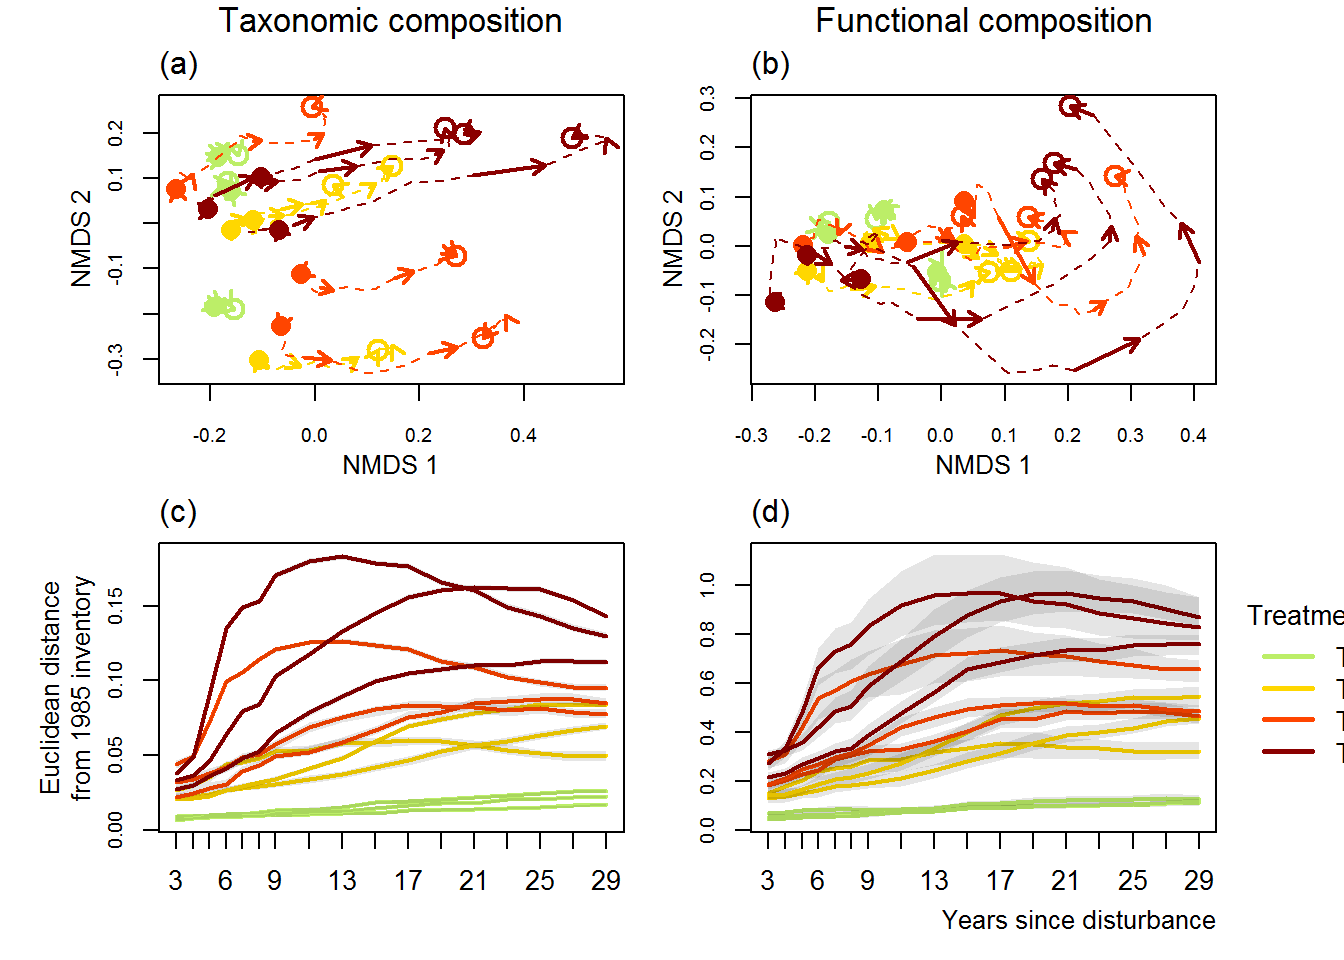
\includegraphics[width=1\linewidth]{WholePlotTrajectories_files/figure-latex/NMDSplans-1} 

}

\caption{Plot trajectories in terms of taxonomic composition (\textbf{(a)} and \textbf{(c)}) and functional composition (\textbf{(b)} and \textbf{(d)}) in a two-dimensional NMDS plan. Lower panels (\textbf{(c)} and \textbf{(d)}) represent the Euclidean distance to initial condition along the 30 sampled years. Shaded areas are the credibility intervals.}\label{fig:NMDSplans}
\end{figure*}

Community CWM average value of all traits and seed mass proportions
followed unimodal trajectories, either stabilizing or returning towards
their initial values, to the exception of leaf chlorophyll content,
which continued to increase for some T3 and T2 plots 30 years after
disturbance.

Community CWM average value of Maximum height at adult stage
(\emph{Hmax}), leaf toughness and wood specific gravity (\emph{WSG})
first decreased and then slightly increased but remained significantly
lower than their initial value (Fig. \ref{fig:CWM}). On the other side,
bark thickness and specific leaf area (\emph{SLA}) increased and while
bark thickness remained substantially high after 30 years, \emph{SLA}
had almost recovered to its initial value. For all traits, the maximum
difference to initial value was correlated to the disturbance intensity.
Positive correlations were observed for Leaf thickness, chlorophyll
content, SLA and bark thickness
(\(\rho_{Spearman}^{Leaf thickness}=0.76\),
\(\rho_{Spearman}^{Chlorophyll content}=0.60\),
\(\rho_{Spearman}^{SLA}=0.93\),
\(\rho_{Spearman}^{Bark thickness}=0.71\)). Negative correlation was
observed for Leaf toughness, WSG and Hmax
(\(\rho_{Spearman}^{Leaf toughness}=-0.53\),
\(\rho_{Spearman}^{WSG}=-0.75\), \(\rho_{Spearman}^{Hmax}=-0.40\)) The
proportions of the three lightest seed mass classes increased in all
disturbed plots, and decreased after 30 years for the lightest class
while it stabilized for the two other (Supp. Mat. - Fig. S2).

\begin{figure*}

{\centering 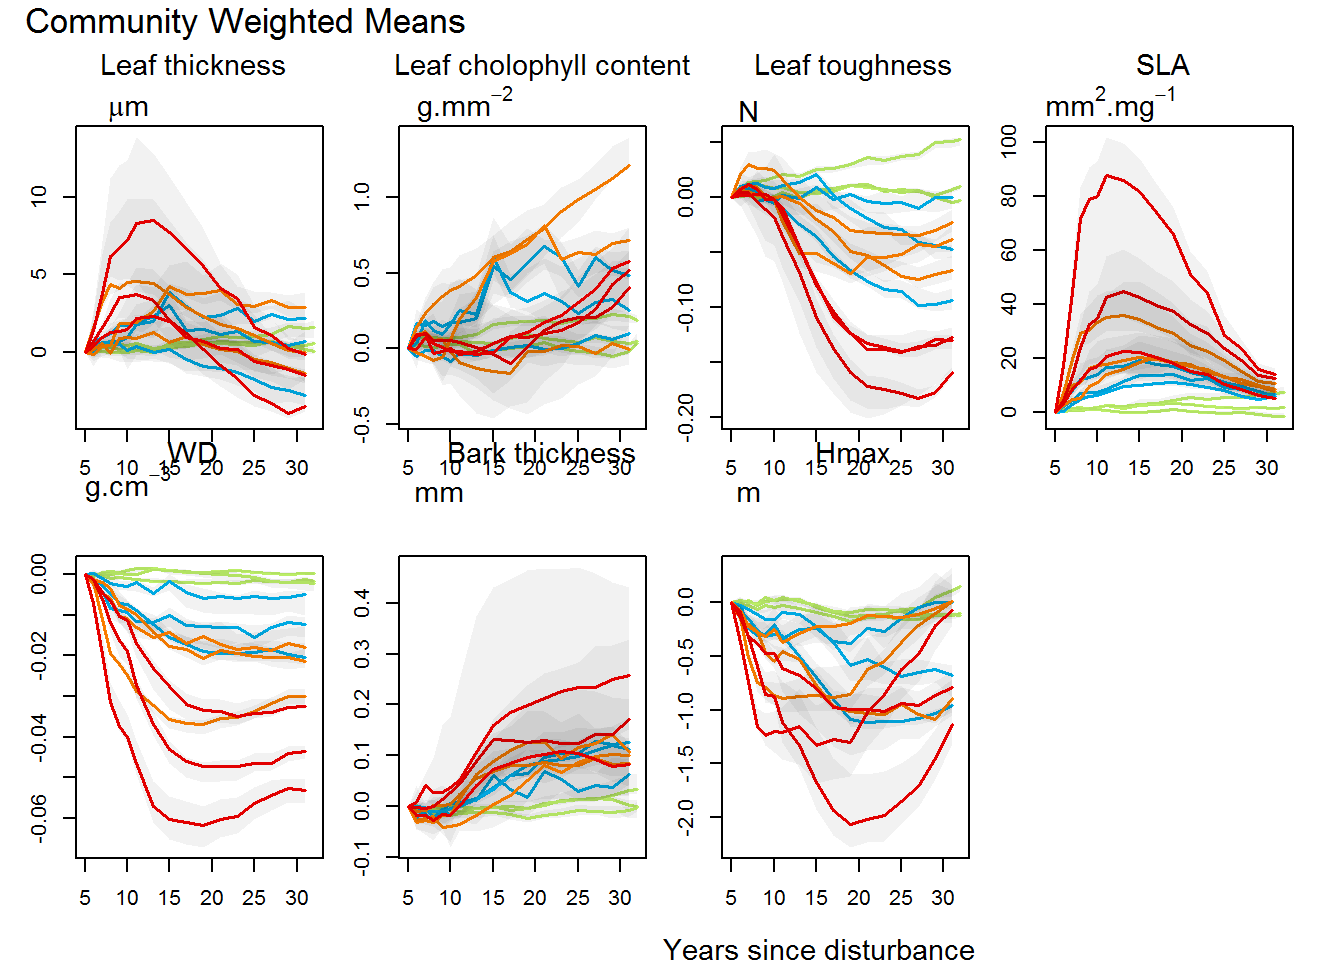
\includegraphics[width=1\linewidth]{WholePlotTrajectories_files/figure-latex/CWM-1} 

}

\caption{Trajectories of community weighted means over 30 years after disturbance of four leaf traits (Leaf thickness, chlorophyll content, toughness, and specific area), two stem traits (wood specific gravity, and bark thickness) and one life history trait (Specific maximum height at adult stage). }\label{fig:CWM}
\end{figure*}

\subsection{Community taxonomic and functional
diversity}\label{community-taxonomic-and-functional-diversity}

For undisturbed plots, taxonomic richness and Simpson diversity remained
stable over the 30 years of monitoring. In disturbed communities, after
low disturbance intensity the taxonomic richness increased, reaching a
maximum gain of 14 botanical genera (plot 3 from treatment 2). After
intense disturbance the taxonomic richness followed a more complex
trajectory, decreasing for ten years after disturbance before recovering
to pre-disturbance values. The maximum richness loss or gain after
disturbance was positively correlated with the disturbance intensity
(\(\rho_{Spearman}^{Richness}=0.50\)). In all disturbed plots the
Simpson diversity first increased until a maximum reached after around
20 years. This maximum was positively correlated with the disturbance
intensity (\(\rho_{Spearman}^{Simpson}=0.77\)). The Simpson diversity
then stabilized except for two T3 plots (plots 8 and 12) for which it
kept increasing (Fig. \ref{fig:DivTaxo}).

\begin{figure*}

{\centering 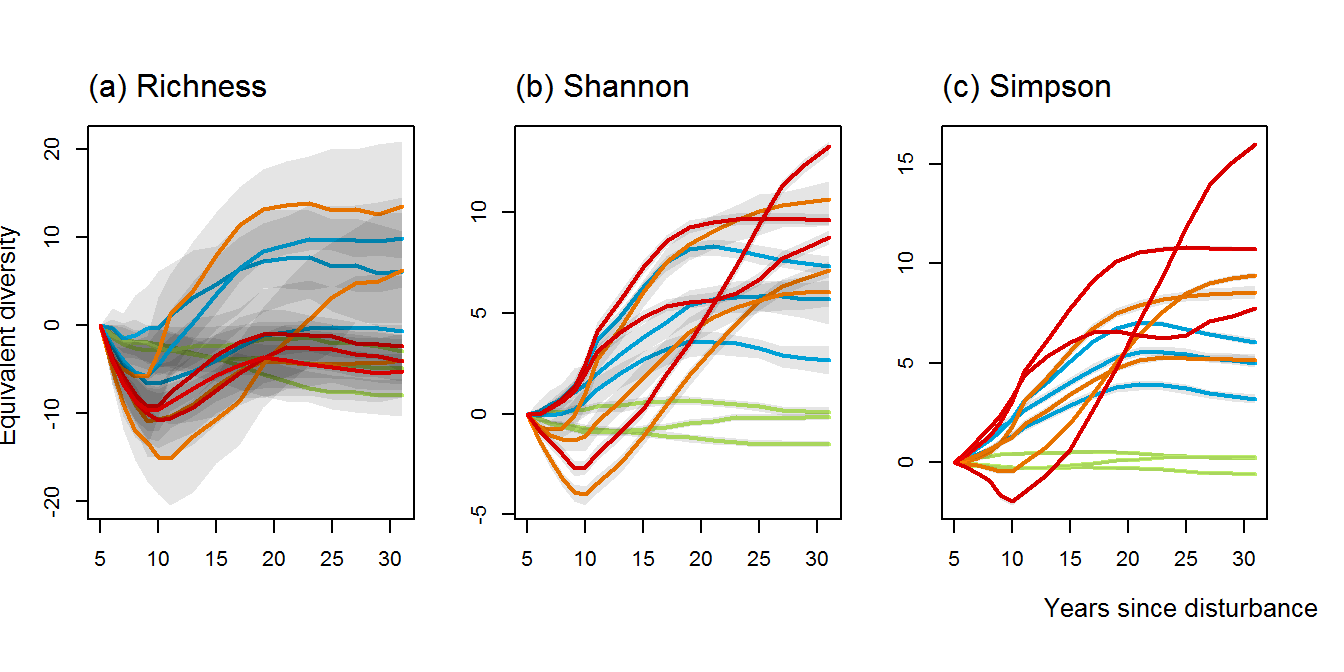
\includegraphics[width=1\linewidth]{WholePlotTrajectories_files/figure-latex/DivTaxo-1} 

}

\caption{Trajectories over 30 years of the difference with the 1989 inventory (2 years after disturbance) of community taxonomic richness \textbf{(a)}, Simpson diversity \textbf{(b)}, functional richness \textbf{(c)}, and Rao diversity \textbf{(d)}. Shaded areas are the credibility intervals }\label{fig:DivTaxo}
\end{figure*}

The plot 7 from treatment 1 displayed constantly outlying functional
richness and Rao diversity and was removed from the graphical
representation for better readability. In undisturbed plots both
functional richness and Rao diversity remained stable along the 30
years. In disturbed plots, both trajectories depended on the disturbance
intensity, with their maximum being positively correlated to \%AGB loss
\(\rho_{Spearman}^{Richness}=0.76\) and \(\rho_{Spearman}^{Rao}=0.60\).
Functional richness and Rao diversity displayed for low disturbance
intensity a low but long-lasting increase up to a maximum reached after
20-25 years, and for high intensity, a fast but short increase followed
after 10 years by a slow decrease towards the initial values.

The second-degree polynomial regressions between (i) the percentage AGB
loss and (ii) taxonomic and functional diversity after 10, 20 and 30
years best predicted the hump-shaped curve of the disturbance impact
along the disturbance intensity gradient \ref{fig:IDHplot}. The
relationship between the disturbance impact and its intensity was more
markedly hump-shaped for the taxonomic richness than for the Simpson
diversity. For both functional richness and Rao diversity the
relationship was almost linear. The regression model better predicted
the functional richness and Rao diversity
(\(0.55<R^2_{Functional Richness}<0.72\), and
\(0.60<R^2_{Functional Rao}<0.81\)) than the taxonomic richness and
evenness (\(0.21<R^2_{Taxonomic Richness}<0.4\), and
\(-0.15<R^2_{Taxonomic Simpson}<0.43\) respectively).

\begin{figure*}

{\centering 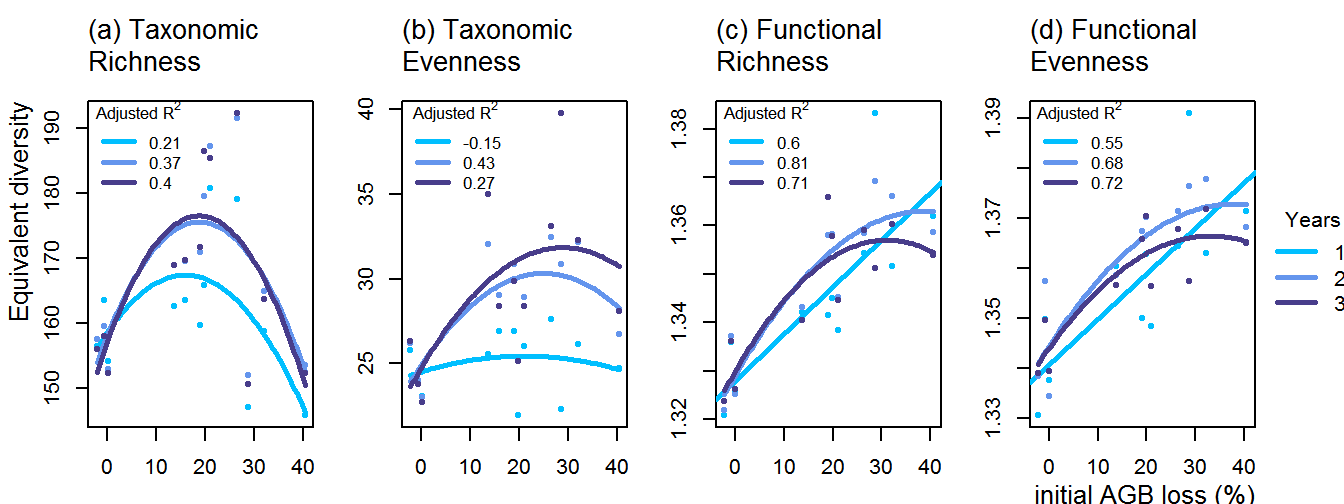
\includegraphics[width=1\linewidth]{WholePlotTrajectories_files/figure-latex/IDHplot-1} 

}

\caption{Relationship between the initial \%AGB loss and community taxonomic richness \textbf{(a)}, taxonomic evenness \textbf{(b)}, functional richness \textbf{(c)},and functional evenness \textbf{(d)} at 10, 20 and 30 years after disturbance}\label{fig:IDHplot}
\end{figure*}

\subsection{Functional redundancy}\label{functional-redundancy}

All disturbed plots had lower functional redundancy than control plots
and followed similar hump-shaped trajectories (\ref{fig:RedFunRest}).
The maximum redundancy loss was positively correlated with the
disturbance intensity (\(\rho_{Spearman}=0.47\)) and the recovery had
not attained initial values for any disturbed communities after 30
years.

\begin{figure}

{\centering 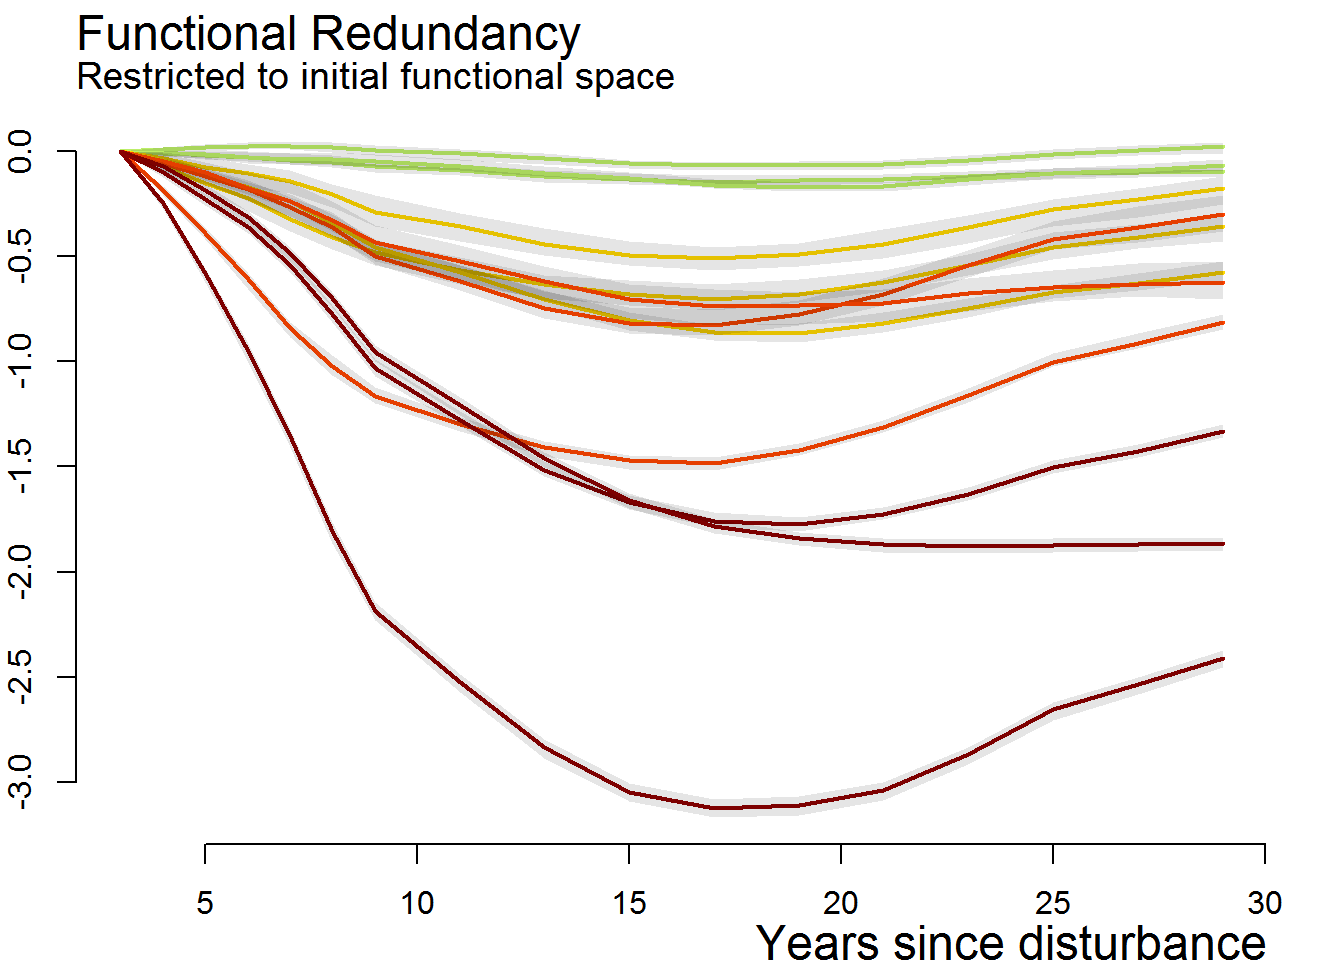
\includegraphics[width=1\linewidth]{WholePlotTrajectories_files/figure-latex/RedFunRest-1} 

}

\caption{Trajectories of the functional redundancy within the initial functional space over 30 years after disturbance. Shaded areas are the credibility intervals.}\label{fig:RedFunRest}
\end{figure}

\section{Discussion}\label{discussion}

\subsection{A cyclic recovery of community
composition}\label{a-cyclic-recovery-of-community-composition}

Community taxonomic and functional composition appeared resilient,
following similar hump-shaped trajectories starting to return towards
pre-disturbance composition after 30 years.

The taxonomic differences among local communities were already apparent
before disturbance, as revealed by the distinct starting points on the
NMDS axis 2. These differences were maintained throughout recovery
trajectories.\\
More than commonly thought, post-disturbance trajectories depended on
community initial composition, which partly determined the pool of
recruited species and constrained the trajectories towards the initial
composition. The community taxonomy proved highly resilient, as it
absorbed the disturbance and maintained commnity initial composition
characteristics \citep{Folke2006}. This high resilience suggested that
species not belonging to the pre-disturbance community were rarely
recruited because of the commonness of dispersal limitation among
tropical tree species \citep{Svenning2005}.

Conversely, disturbed communities followed functional trajectories that
are highly similar in terms of functional composition. As the
composition of pre-disturbance surviving trees is representative of the
initial community \citep{Herault2018}, changes in functional composition
relied upon the recruitment of species or functional types that were
infrequent or absent before disturbance. Competitive pioneers became
dominant in filling the environmental niches of high availability of
light, space and nutrients vacated by the disturbance. The recruitment
of pioneers changed community functional composition in the same way for
all disturbance intensity towards more resource-acquisitive strategies,
moving community functional composition right along the first axis in
Fig. \ref{fig:NMDSplans} \citep{Westoby1998, Wright2004, Reich2014}.
Thereafter long-lived, more resistant and shade-tolerant species
excluded the first established pioneers and started the recovery of
pre-disturbance functional composition, moving similarly community
functional composition left along the first axis and upward along the
second axis in Fig. \ref{fig:NMDSplans}.

These trajectories provided empirical support to the hypothesis that
community assembly is both deterministic and historically convergent at
different levels of community organization. Deterministic, trait-based
processes drove community convergence in functional composition, while
at the same time dispersal limitation maintained their divergence in
taxonomic composition \citep{Fukami2005}.

\subsection{A new perspective on the intermediate disturbance
hypothesis}\label{a-new-perspective-on-the-intermediate-disturbance-hypothesis}

Community taxonomic richness increased after disturbance until an
intensity threshold (20-25\% AGB loss) above which the taxonomic
richness decreased. The increase of taxonomic evenness after disturbance
also depended on the disturbance intensity, although the correlation was
weaker than for the taxonomic richness as already observed in the Guiana
Shield \citep{Baraloto2012a} and in Bornean tropical forests
\citep{Cannon1998}. In accordance with the IDH, then, community
taxonomic trajectories depended on the disturbance intensity. They
markedly changed above an intensity threshold, with a decrease of the
richness and a persistent increase of the evenness. Disturbance
intensity determined the balance in the community between surviving
trees from pre-disturbance communities and trees recruited afterward.
The pool of true pioneer species specifically recruited after
disturbance is, in the Guiana Shield, restricted to a few common genera
(e.g. \emph{Cecropia} spp., \emph{Vismia} spp.)\citep{Guitet2018}. Below
the intensity threshold the surviving community trees remained numerous
enough to maintain the pre-disturbance high taxonomic richness while the
pioneers recruited, infrequent or absent before disturbance, increased
both community taxonomic richness and evenness. Beyond the intensity
threshold, disturbance decreased the taxonomic richness of surviving
trees, and this decrease was not offset by the recruitment of pioneers.
The overall community taxonomic richness therefore decreased according
to the disturbance intensity \citep{Molino2001}. An intermediate
disturbance was then detected, defined by an intensity for which
post-disturbance trajectories markedly changed. Such disturbance
increased the availability of resources and created opportunities for
pioneers, without implying too important loss of shade-tolerant species
or preventing their maintenance in the community \citep{Bongers2009}.
For community taxonomic evenness, the disturbance impact was similar but
milder. Because the evenness is less sensitive to the loss of rare
species, below the intensity threshold the trajectories of taxonomic
evenness rather represented the increasing dominance of pioneers that
balancing the usual hyper-dominance of a few species. Beyond the
intensity threshold, however, pioneers became in turn highly dominant
and decreased the overall evenness \citep{Baraloto2012a}.

Conversely the IDH was disproved regarding the disturbance impact on
community functional richness and evenness. Irrespective of the
disturbance intensity, both community functional richness and evenness
increased following the recruitment of pioneers, functionally highly
different from the composition of pre-disturbance community.

Along time, taxonomic richness trajectories of all disturbed communities
similarly dropped at first place, following the species loss due to
disturbance, and then displayed a species gain depending on the
disturbance intensity. Up to an intensity threshold, the species gain
was all the more significant that the disturbance intensity increased,
with the establishment of long-lived pioneers enhancing community
taxonomic richness and evenness in the long term. These long-lived
pioneers, functionally quite different from the functional composition,
entailed as well a progressive and long-lasting increase of the
functional richness and evenness \citep{Denslow1980, Molino2001}. Beyond
an intensity threshold, though, a few short-lived pioneers occupied the
vacated environmental space and prevented the establishment of other
species. These short-lived pioneers were functionally very different
from the pre-disturbance community and entailed a rapid and significant
increase of functional richness and evenness. Already after 10 years,
though, short-lived pioneers started to decline and the functional
richness and evenness decreased. Likely this decrease will be followed
by the establishment of long-lasting pioneers, and by the time they
recruit we expect the taxonomic and functional trajectories to catch up
with those observed after intermediate disturbance \citep{Walker2009}.

\subsection{The functional redundancy, key of community
resilience}\label{the-functional-redundancy-key-of-community-resilience}

For 15 years the species loss during disturbance, determined by the
disturbance intensity, significantly decreased the functional redundancy
within the pre-disturbance functional space. The redundancy decrease was
not compensated for in the first place as the first recruited pioneers
were functionally different from the pre-disturbance functional
composition. Progressively though, first established species were
replaced by more competitive long-lived pioneers or late-successional
species resembling more the pre-disturbance functional composition and
restoring the functional redundancy. This replacement was stochastic and
followed the lottery recruitment rules, implying a recruitment eased for
the first recruited species but then increasingly hampered by the
emergence of interspecific competition \citep{Busing2002}. Along time
the recovery of infrequent species was increasingly slow, so that the
time to full recovery of the functional redundancy, in some communities
just initiated after 30 years, was extremely difficult to estimate
\citep{Elmqvist2003, Diaz2005}.

The mid-term impact of disturbance on community functional redundancy
meant a lower resilience of the pre-disturbance communities, with higher
chances to see the persistence of disturbance-specific species at the
expense of late-successional ones \citep{Haddad2008}. Besides, the
mid-term recovery of infrequent species increases the risks to loose
keystone species, with unexpected ecological consequences
\citep{Jones1994, Chazdon2003a, Diaz2005}. Apart from the functional
characteristics considered here, infrequent species might indeed have
unique functions in the ecosystem or be a key for some fauna
\citep{Schleuning2016}.

\section{Conclusions}\label{conclusions}

Our study revealed community recovery through the combination of
deterministic processes driving their convergence in functional
composition, and dispersal limitation maintaining their divergence in
taxonomic composition. The IDH was validated for community taxonomic
richness and, to some extent, taxonomic evenness but disproved regarding
community functional richness and evenness which were enhanced for any
disturbance intensity by the high functional differences of pioneers
compared to late-successional functional composition. The IDH was
translated in time by the recruitment, beyond an intensity threshold, of
short-lived pioneers that prevented in the first years after disturbance
the establishment of more diverse long-lived pioneers, recruited
otherwise below the intensity threshold. The resilience of tropical
forests, defined in terms of recovery to pre-disturbance state, proved
tangible but requiring several decades. Still, the disturbance impact on
community redundancy cautioned against the risks of infrequent species
loss and the persistence of disturbance-specific communities
\citep{Herault2018}.

\section{Acknowledgement}\label{acknowledgement}

We are in debt with all technicians and colleagues who helped setting up
the plots and collecting data over years. Without their precious work,
this study would have not been possible and they may be warmly thanked
here.

\section{Author's contributions}\label{authors-contributions}

AM, EM \& BH designed the study, developed the analysis framework,
interpreted the results and wrote the manuscript. All authors gave final
approval for publication.

\section{Data availability}\label{data-availability}

This article is based upon the dataset of the Paracou station, which is
part of the Guyafor permanent plot network in French Guiana
(Cirad-CNRS-ONF). The dataset is available upon request to the
scientific director (https://paracou.cirad. fr).

%----------------------------------------------------------------------------------------
%	REFERENCE LIST
%----------------------------------------------------------------------------------------

\bibliographystyle{mee}
\makeatletter
% The filename has .bib extension the must be eliminated
\filename@parse{references.bib}
% parse stores the file name in base. Extension starts at the first dot, so don't use dots in file names.
\bibliography{\filename@base}
\makeatother


%----------------------------------------------------------------------------------------

\end{document}
